\begin{problem}{Rebuild binary tree}{standard input}{standard output}{1 second}{256 megabytes}

Level order traversal is visiting nodes by visiting nodes at each depth level from left to right, before moving to the next depth level.

Inorder traversal is visiting nodes by first visiting the left subtree, then processing the current node, and finally visiting the right subtree.

For the example graph (sample test 1) below:
\begin{itemize}
\item level order traversal: 1 2 7 3 4 8 5 6 9
\item inorder traversal: 3 2 5 4 6 1 7 9 8
\end{itemize}

\begin{center}
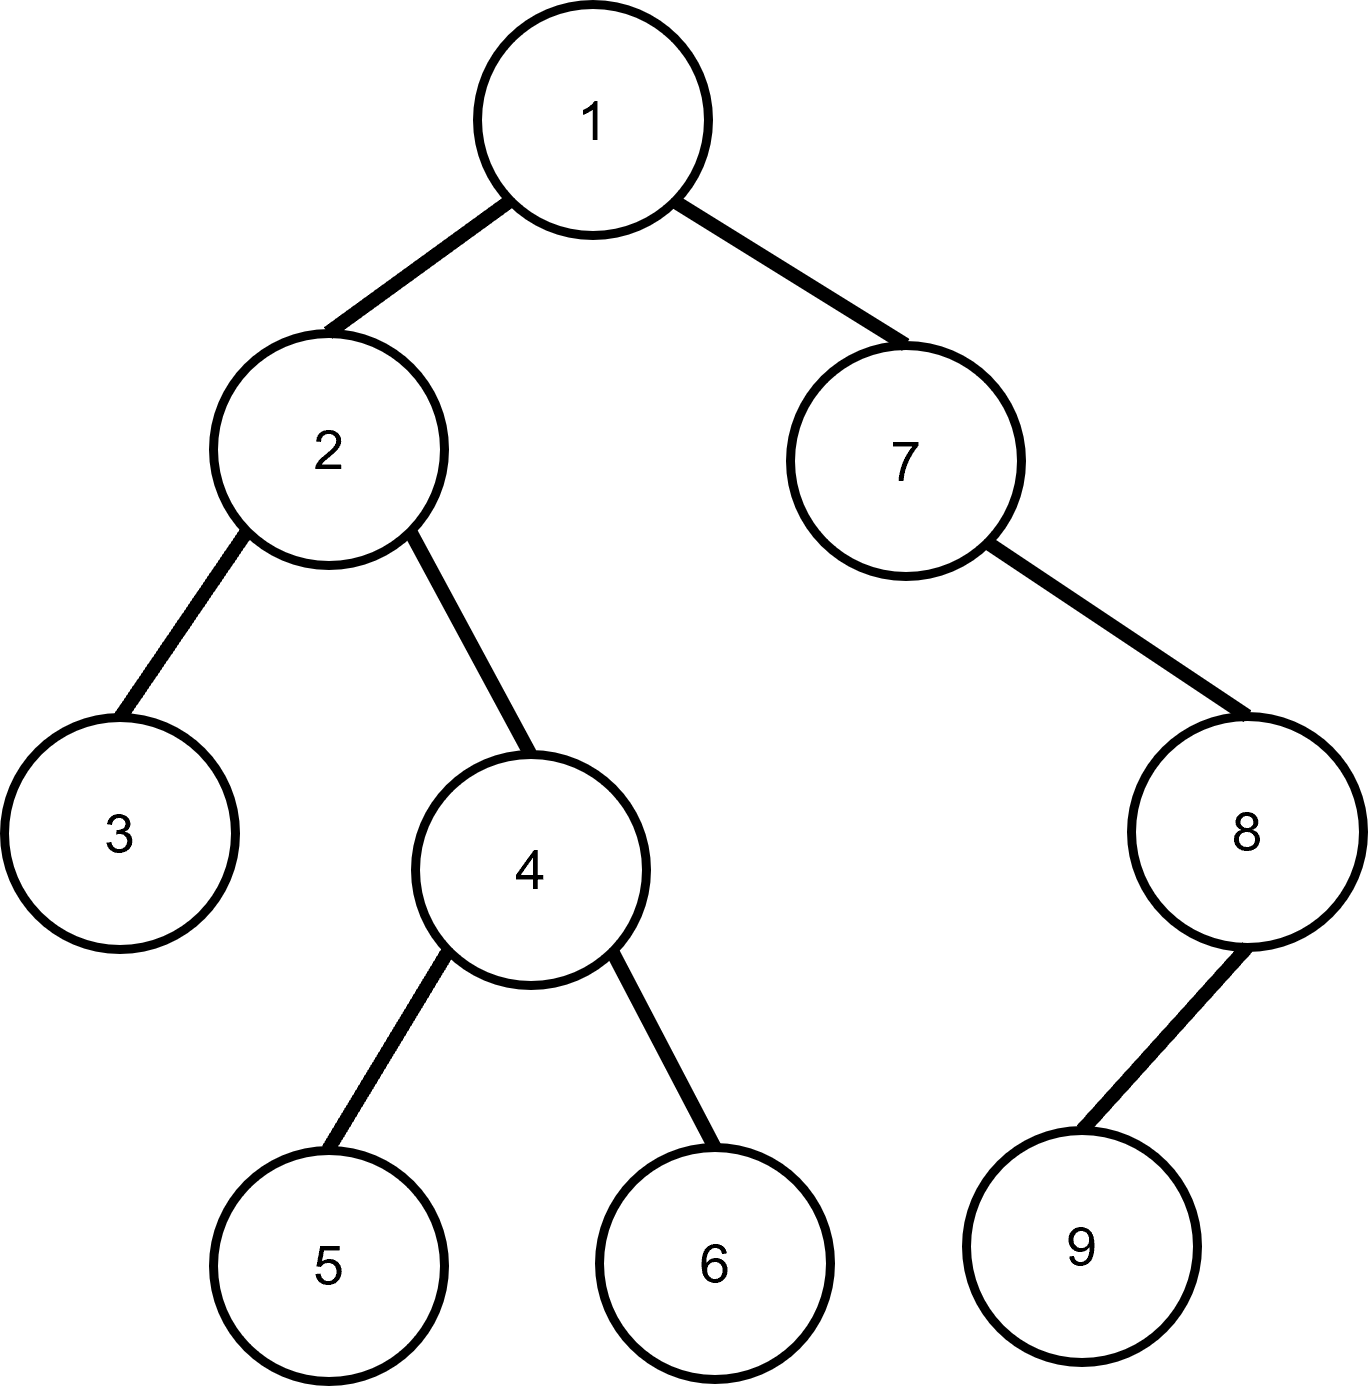
\includegraphics[scale=0.25]{binarytree.png}
\end{center}

Given the level order traversal and inorder traversal of a binary tree, your task is to rebuild the binary tree.

\InputFile
The first line of the input contains an ineger $n$ ($1\le n\le 10^5$) --- the number of nodes in the binary tree.

The second line of the input contains $n$ integers --- the level order traversal of the tree.

The last line of the input contains $n$ integers --- the inordre traversal of the tree.



\OutputFile
You should print $n$ lines.

For the $i$-th line, you should print two integers $l_i, r_i$ --- the left child of $i$ and the right child of $i$.

If the node doesn't exist, print 0 instead.




\Examples

\begin{example}
\exmpfile{example.01}{example.01.a}%
\exmpfile{example.02}{example.02.a}%
\end{example}

\Note
The root is not necessarily $1$.

    
    
\end{problem}
    